\chapter{The Renormalization Group}
\section[The Wilsonian Renormalization Group]{The Wilsonian Renormalization Group\footnote{P \& S, Ch 12.1}}
We will study influence of UV fluctuations more explicitly using UV cutoff $\Lambda$. It is difficult for gauge theories, but more intuitive for $\phi^4$.

Consider path integral with field vanishes in momentum space,
\begin{align*}
   Z[J] &= \int [\D \phi] \exp{i\int \dd[4]{x} (\lag + \phi J)} \\
        &= \prod_k \int \dd{\phi(k)}  \exp{i\int \dd[4]{x} (\lag + \phi J)}
\end{align*} 
We would like to separate out integration over modes with $|k| \leq \Lambda$. It is difficult in Minkowski space, since Minkowski "scalar product" is not positive semi-definite. So first perform Wick rotation to Euclidean space, where momentum cutoff $\Lambda$ is well defined. Euclidean path integral
\begin{align}
   \eval{Z_E[J]}_{J=0} &= \int [\D \phi]_\Lambda \exp{-\int \dd[d]{x_E} \left(\frac{1}{2} ( \partial \phi)^2 + \frac{1}{2} m^2 \phi^2 + \frac{\lambda}{4!}\phi^4 \right)}
\end{align}
Drop the subscript $E$ from now on. $m$ and $\lambda$ are bare parameters, there are no counter-terms yet. Dimension $d$ to keep discussion general.

Idea is to lower the cutoff $\Lambda$ somewhat, from $\Lambda \rightarrow b \Lambda$, with b a small positive number $ 0 < b < 1$. 
\paragraph{Define} \underline{low- and high-momentum modes} 
\begin{align}
   \tilde{\phi}(k) &= \begin{cases} \phi(k) & |k| \leq b \Lambda  \\ 0 &  |k| > b\Lambda \end{cases} \\
   \hat{\phi}(k) &= \begin{cases} 0 & |k| \leq b \Lambda \\ \phi(k) & b \Lambda < |k| \leq \Lambda \end{cases}
\end{align}
so that field can be decomposed into low-momentum modes and high-momentum modes.
\begin{align}
   \phi(k) = \tilde{\phi}(k) + \hat{\phi}(k) 
\end{align}
Rename low-momentum mode $\tilde{\phi}(k) = \phi(k)$.

In the path integral $[\D \phi]_{\Lambda} = [\D \phi]_{b \Lambda} [\D \hat{\phi}]$ and substitute $\phi \mapsto \phi + \hat{\phi}$ in the Lagrangian.
\begin{align*}
   Z &= \int [\D \phi]_{b \Lambda} \int [\D \hat{\phi}] \exp{ - \int \dd[d]{x} \left[\frac{1}{2} (\partial \phi + \partial \hat{\phi})^2 + \frac{m^2}{2}(\phi + \hat{\phi})^2 + \frac{\lambda}{4!} (\phi + \hat{\phi})^4 \right] } \\
     &=  \int [\D \phi]_{b \Lambda} \exp{- \int \dd[d]{x} \lag [\phi]} \int [\D \hat{\phi}] \exp{ - \int \dd[d]{x} \left[ \frac{1}{2} (\partial \hat{\phi})^2 + \frac{m^2}{2} \hat{\phi}^2 + \lambda \left(\frac{1}{6} \phi^3 \hat{\phi} + \frac{1}{4} \phi^2 \hat{\phi}^2 + \frac{1}{6} \phi \hat{\phi}^3 + \frac{1}{4!} \hat{\phi}^4 \right) \right]}
\end{align*}
Note that terms of order $\phi\hat{\phi}$ vanish! They would contribute to propagator-type terms, not have disjoint momentum support (different Fourier components orthogonal!)

Interaction terms of the form (double line for high momentum modes, single line for low momentum modes)
\begin{align*}
   \feynmandiagram[small, layered layout]{
      i1 -- v-- f1;
      i2 -- v-- f2;
   };\quad 
   \feynmandiagram[small, layered layout]{
      i1 -- v--[double] f1;
      i2 -- v-- f2;
   };\quad 
   \feynmandiagram[small, layered layout]{
      i1 -- v--[double] f1;
      i2 -- v--[double] f2;
   };\quad 
   \feynmandiagram[small, layered layout]{
      i1 --[double] v--[double] f1;
      i2 -- v--[double] f2;
   };\quad 
   \feynmandiagram[small, layered layout]{
      i1 --[double] v--[double] f1;
      i2 --[double] v--[double] f2;
   };
\end{align*}

After $\int \D \hat{\phi}$ path integral is carried out, the generating function should look like
\begin{align*}
   Z \stackrel{!}{=} \int [\D \phi]_{b \Lambda} \euler^{-\int \dd[d]{x} \lag_\text{eff}(\phi)}
\end{align*}
Now $\lag_\text{eff}$ only involves Fourier components with $|k| \leq b \Lambda$.

How does $\lag_\text{eff}$ look like?
\begin{align}
   \lag_\text{eff} = \lag(\phi) + \text{corrections}
\end{align}
The corrections are in order of $\lambda$. The correction terms compensate for the removal of high-momentum Fourier components/fluctuations in $\hat{\phi}$.

We are interested in large-ish cutoffs $\Lambda^2 \gg m^2$. Treat $m^2$ and $\lambda$ terms in the $\D \hat{\phi}$ path integral as perturbations. Leading propagator comes from
\begin{align*}
   \int \dd[d]{x} \lag_0 &= \int \dd[d]{x} \frac{1}{2} (\partial \hat{\phi})^2 \\
                         &= \int \frac{\dd[d]{k}}{(2\pi)^d} \frac{1}{2} \hat{\phi}^*(k) k^2 \hat{\phi}(k)
\end{align*}

The contraction is similar to a normal propagator 
\begin{align}
   \bcontraction{}{\hat{\phi}}{(k)}{\hat{\phi}} \hat{\phi} (k) \hat{\phi} (p) = \frac{\int \D \hat{\phi} \hat{\phi}(k) \hat{\phi} (p) \euler^{-\int \dd[d]{x} \lag}}{\int \D \hat{\phi} \euler^{-\int \dd[d]{x}\lag_0 }} \notag \\
   = \frac{1}{k^2} (2\pi)^d \delta^{(d)}(p + k) \hat{\theta}(k)  \label{math:phiphi}
   \shortintertext{where}
   \hat{\theta}(k) = \begin{cases} 1 & b \Lambda < |k| \leq \Lambda \\ 0 & \text{otherwise} \end{cases} \notag
\end{align}

Perturbations in $m^2$ and $\lambda$ are calculated expanding the exponential, using Wick's theorem with propagator from above. What corrections in $\lag_\text{eff}$ will the $\hat{\phi}$ field generate?

\paragraph{Tree level diagrams} 
Diagram with $\phi^3 \bcontraction{}{\hat{\phi}}{\phi^3}{\hat{\phi}} \hat{\phi} \phi^3 \hat{\phi}$
\begin{align*}
   \feynmandiagram[baseline=(v1.base), small, horizontal=v1 to v2, layered layout]{
      {i1[particle=\(p_1\)], i2[particle=\(p_2\)], i3[particle=\(p_3\)]} -- v1 --[double] v2 -- {f1[particle=\(p_1\)], f2[particle=\(p_2\)], f3[particle=\(p_3\)]};
   };
   \sim \frac{\lambda^2}{(p_1 + p_2+ p_3)^2} \hat{\theta} (p_1 + p_2 + p_3)
\end{align*}
does not contribute for $p_1, p_2, p_3 \ll \Lambda^2$. Similarly other tree-level diagrams won't contribute.

Consider $p_i = 0$ (external) for now!

\paragraph{Single $\hat{\phi}$ loop}
\begin{align*}
   
\includegraphics[width=0.8\linewidth]{./RG/1.eps}
\end{align*}

Calculate $(1)$ explicitly using equation (\ref{math:phiphi})
\begin{align*}
   (1) = -\frac{\lambda}{4}  \int \dd[d]{x} \phi^2 \bcontraction{}{\hat{\phi}}{}{\hat{\phi}} \hat{\phi} \hat{\phi} &=: - \frac{1}{2}\int \frac{\dd[d]{k_1}}{(2\pi)^d} \Delta m^2 \phi(k_1) \phi(-k_1)  \\
\end{align*}
in which 
\begin{align*}
   \Delta m^2 &= \frac{\lambda}{2} \int_{b \Lambda < |k| \leq \Lambda} \frac{\dd[d]{k}}{(2\pi)^d} \frac{1}{k^2} \\
              &= \frac{\lambda}{2} \frac{\Omega_d}{(2\pi)^d} \int_{b \Lambda}^\Lambda \dd{k} k^{d-3} \\
              &= \frac{\lambda}{(4\pi)^{d/2}} \frac{1}{\Gamma (d/2)} \frac{\Lambda^{d-2}}{d-2} (1- b^{d-2})
   \shortintertext{with $n$ dimensional solid angle $\Omega_d = 2 \pi^{d/2} / \Gamma(d/2)$. In $d=4$}
   \Delta m^2 &= \frac{\lambda}{16 \pi^2} \frac{\Lambda^2}{2} (1-b^2)
\end{align*}
 Remember $b < 1$ so $\Delta m^2 > 1$.

Second diagram give $- \frac{\Delta \lambda}{4!} \phi^4$ in effective Lagrangian. Setting external momenta to zero
\begin{align*}
   \Delta \lambda &= - 4! \frac{2}{2!} \left(\frac{\lambda}{4}\right)^2 \int \frac{\dd[d]{k}}{(2\pi)^d} \left( \frac{1}{k^2} \right)^2  \\
                  &= - \frac{3}{2} \lambda^2 \frac{2}{(4\pi)^{d/2} \Gamma(d/2)} \int_{b \Lambda}^{\Lambda} \dd{k} k^{d-5} \\
                  &= \frac{-3 \lambda^2}{(4\pi)^{d/2} \Gamma(d/2)} \frac{\Lambda^{d-4}}{d-4} (1-b^{d-4})  \\
                  &= - \frac{3 \lambda^2}{16 \pi^2} \ln( \frac{1}{b})
\end{align*}
It's negative since $0 < b < 1$!

If we set external momenta $p_i \neq 0$: Taylor expand in $p_i$,  it will generate interactions terms $(\partial \phi)^2 \phi^2$, $(\partial \phi)^4$, $\dots$.

Third diagram generates term $\sim \lambda^3 \phi^6$ (in $d=4$, $\propto \frac{\lambda^3 \phi^6}{\Lambda^2}$). Higher dimensional, non-renormalizable interactions are generated! We will see soon why it is not a real problem.

\paragraph{Comments}
\begin{itemize}
   \item Everything is finite, although being cutoff-dependent
   \item Is loop expansion $\frac{\lambda + \Delta \lambda}{4!} \phi^4$ valid?
      \begin{align*}
         \lambda + \Delta \lambda = \lambda \bigg[ 1- \underbrace{\frac{3\lambda}{16 \pi^2} \ln(1/b)}_{\ll 1} \bigg]
      \end{align*}
      Higher order ($N$ loops) will scale like $\lambda (\frac{\lambda}{16\pi^2} \ln(1/b))^N$. 
      \begin{align*}
         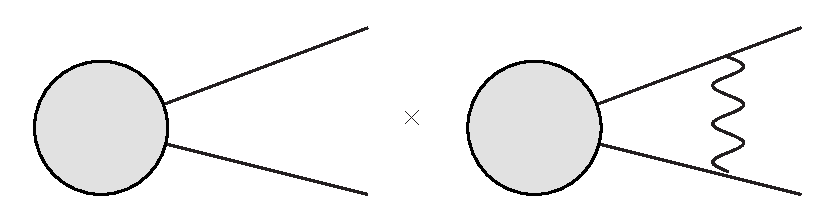
\includegraphics[width=0.4\linewidth]{./RG/2.eps} 
      \end{align*}
      It is even smaller corrections.
\end{itemize}

More careful comparison of $\lag $ and $ \lag_\text{eff}$
\begin{align*}
   Z &= \int [\D \phi]_{b \Lambda} \euler^{- \int \dd[d]{x} \lag_\eff} \\
   \lag_\text{eff} &= \frac{1}{2} (1 + \Delta Z) (\partial \phi)^2 + \frac{1}{2} (m^2 + \Delta m^2) \phi^2 + \frac{1}{4!} (\lambda + \Delta \lambda) \phi^4 + \Delta C ((\partial \phi)^2)^2 + \Delta \tilde{C} \phi^2 (\partial \phi)^2 + \Delta D \phi^6 + \dots
\end{align*}

Now rescale distances and momenta $k' = k / b$ or $x' = xb$. $k'$ in integrated up to $\Lambda$ (original cutoff).
\begin{align*}
   \int \dd[d]{x} \lag_\eff &= \int \dd[d]{x'} b^{-d} \bigg[ \frac{1}{2} (1+\Delta z) b^2 (\partial' \phi)^2 + \frac{1}{2} (m^2 + \Delta m^2)\phi^2 \\
      &+ \frac{1}{4!} (\lambda + \Delta \lambda) \phi^4 + \Delta C b^4 (\partial \phi)^4 + \tilde{\Delta C}b^2 (\partial' \phi)^2 \phi^2 + \Delta D \phi^6 + \dots \bigg]
\end{align*}
Now rescale the fields  
\begin{align*}
  \phi' = \sqrt{b^{2-d} (1+ \Delta Z)} \phi 
\end{align*}
to obtain canonical kinetic term
\begin{align*}
      \int \dd[d]{x} \lag_\eff &= \int \dd[d]{x'} \left[ \frac{1}{2} (\partial' \phi')^2 + \frac{1}{2} m'^2 \phi'^2 + \frac{1}{4!} \lambda' \phi'^4 + C' (\partial' \phi')^4 + \tilde{C}' (\partial' \phi')^2 \phi'^2 + D' \phi'^6 \right]
\end{align*}
with the scaled variables
\begin{align*}
   m'^2 &= \frac{m^2 + \Delta m^2}{b^2(1+\Delta Z)} \\
   \lambda' &= \frac{\lambda + \Delta \lambda}{b^{4-d} (1+ \Delta Z)^2} \\
   C' &= b^d \frac{C+ \Delta C}{(1+\Delta Z)^2} \\
   \tilde{C}' &= b^{d-2} \frac{\tilde{C} + \Delta \tilde{C}}{(1+\Delta Z)^2} \\
   D' &= b^{2d-6} \frac{D+ \Delta D}{(1+\Delta Z)^3}
\end{align*}
Even if we had $C = \tilde{C} = D = 0$ initially, it would apply as well.

So combination of integrating out degree of freedom and rescaling leads to transformation of $\lag$ (with identical $Llamba$). $\lag$ characterized by set of coupling constants 
\begin{align*}
  (m^2, \lambda, C, \tilde{C}, D, \dots) \mapsto (m'^2, \lambda', C', \tilde{C}', D', \dots) 
\end{align*}

This operation can be repeated, make it infinitesimal $ b \mapsto 1 - db$, so that it's continuous. Transformation in space of all possible Lagrangians.

Study trajectory or flows leads to Renormalization Group. It is not really a group, rather a semi-group, as transformation of "integrating-out" high-momentum degree of freedom is not invertible.

Two possible ways to perform calculations of correlation functions for $|p_i| \ll \Lambda$ 
\begin{itemize}
   \item use original $\lag$, high-momentum fluctuations in loops
   \item use $\lag_\eff$ high-momentum fluctuations have been absorbed in new coupling constants. Already at tree-level. Essentially it is effective field theory.
\end{itemize}

\paragraph{Renormalization Group (RG) in Detail}
Consider $\lag$ near the free theory $m^2 = \lambda =C = \tilde{C} = D = \dots = 0$
\begin{align*}
   \lag_0 = \frac{1}{2} (\partial \phi)^2
\end{align*}
$\lag_0$ is unchanged under the RG flow. It is fixed point.

Near $\lag_0$, only consider terms \underline{linear} in perturbation. Neglect $\Delta m^2 (\propto \lambda), \Delta \lambda (\propto \lambda^2), \Delta Z (\propto \lambda^2), \Delta C, \Delta \tilde{C} (\propto \lambda^2), \Delta D (\propto \lambda^3)$. Then simply have 
\begin{align*}
   m'^2 &= m^2 b^{-2} \\
   \lambda' &= \lambda b^{d-4} \\
   \tilde{C}' &= \tilde{C} b^{d-2} \\
   C' &= C b^d \\
   D' &= D b^{2d-6}
\end{align*}

Since $0 < b < 1$, behaviours are classified as following
\begin{itemize}
   \item \underline{relevant} term grows with RG, 
   \item \underline{marginal} term in $d=4$ unchanged  (higher orders unimportant)
   \item \underline{irrelevant} term diminished in RG flow
\end{itemize}

This can actually be seen directly from dimensional analysis. Operator with $N$ fields $\phi$ and $M$ derivatives scales as 
\begin{align*}
   C'_{N, M} &= b^{N(d/2 - 1) + M - d} C_{N, M} \\
             &= b^{d_{N, M} - d} C_{N, M}
\end{align*}
with $d_{N,M}$ mass dimension of the operator.

Note: relevant/marginal/irrelevant terms correspond to super-renormalizable/renormalizable/non-renormalizable interactions.

One can understand evolution of couplings near a fixed point from dimensional analysis! Near fixed point, arbitrary complicated $\lag$ reduces to a finite number of renormalizable term! (Only near fixed point!)

Illustrate RG flow for $\phi^4$ in 3 cases
\begin{itemize}
   \item \underline{$d > 4$} only mass term is relevant, everything else irrelevant. Only $m^2$ grows, since $m'^2 = m^2 b^{-2n}$ after $n$ iterations. Ultimately $m'^2 \sim \Lambda^2$. Integrate complete momentum range between $\Lambda$ and the effective mass $m'$.
   \item \underline{$d=4$} marginal $\lambda$? Go back to the full transformation including non-linear terms.
      \begin{align*}
         \lambda' = \frac{\lambda + \Delta \lambda}{b^{4-d} (1+\Delta Z)^2} = \lambda - \frac{3\lambda^2}{16\pi^2} \ln(1/b) + \order{\lambda^3}
      \end{align*}
      $\lambda$ slowly decreases as high-momentum modese are integrated out. Coupling goes to zero $\phi^4$ becomes non-interacting in $d=4$.
   \item \underline{$d < 4$} $\lambda$ is relevant! Coupling grows. Non-linear effects are important. 
      \begin{align*}
         \lambda' = b^{d-4} \left[ \lambda = \frac{3\lambda^2}{(4\pi)^{d/2}} \frac{1}{\Gamma(d/2)} \frac{b^{d-4} - 1}{4-d} \Lambda^{d-4} \right]
      \end{align*}
      There is a second fixed point, besides a trivial one $\lambda = 0$.
      \begin{align*}
         \lambda = \frac{4-d}{3} (4\pi)^{d/2} \Gamma(d/2) (\Lambda b)^{4-d} > 0
      \end{align*}
      where the non-linear effects compensate the rescaling!
\end{itemize}
\begin{align*}
   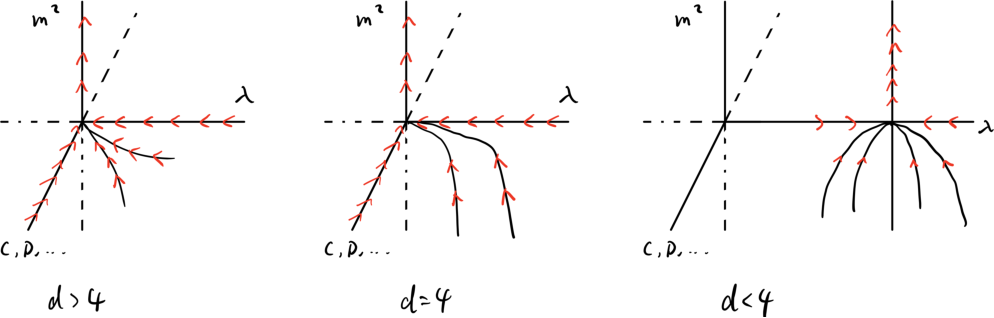
\includegraphics[width=0.8\linewidth]{./RG/RGFlow.pdf}
\end{align*}

\paragraph{Remarks}
\begin{itemize}
   \item for $d<4$ but "close", the new fixed point will be "close" to the free fixed point. Then perturbation theory still make sense. Could have stronly=coupled theories as a fixed point. More difficult, study exactly solvable models.
   \item $m^2 d^2$ im $\phi^4$ always relevant, diverges quickly, naturally $m \mapsto \Lambda$.Problems for theories with elementary scales (Higgs in Standard Model)
\end{itemize}
